\documentclass[conference]{IEEEtran}
\IEEEoverridecommandlockouts
\usepackage{geometry}
\usepackage{graphicx} % Required for inserting images
\usepackage{titlesec}
\usepackage{float}
\usepackage{multirow}
\usepackage{biblatex}
\usepackage{appendix}
\usepackage{amsmath,amssymb,amsfonts}
\usepackage{algorithmic}
\usepackage{pythonhighlight}
\usepackage{graphicx}
\usepackage{mathtools,amssymb,lipsum, caption}
\usepackage{textcomp}
\usepackage{xcolor}
\usepackage{cuted}
\usepackage{listings}
\usepackage{fancyvrb}
\usepackage{framed}
\usepackage[listings,skins]{tcolorbox}
\usepackage[skipbelow=\topskip,skipabove=\topskip]{mdframed}
\mdfsetup{roundcorner=0}
\setlength\stripsep{3pt plus 1pt minus 1pt}
\setcounter{secnumdepth}{5}
\title{Solid Mechanics Report}
\author{boxuan ye}
\date{February 2024}
\addbibresource{reference.bib}
\geometry{margin=1in}
\DeclarePairedDelimiter{\ceil}{\lceil}{\rceil}
\def\BibTeX{{\rm B\kern-.05em{\sc i\kern-.025em b}\kern-.08em
    T\kern-.1667em\lower.7ex\hbox{E}\kern-.125emX}}
\begin{document}

\maketitle
\begin{abstract}
    This document is a model and instructions for \LaTeX.
    This and the IEEEtran.cls file define the components of your paper [title, text, heads, etc.]. *CRITICAL: Do Not Use Symbols, Special Characters, Footnotes, 
    or Math in Paper titles or abstracts.
\end{abstract}

\section{Introduction}
        According to the assumptions, there is no energy lost during the projectile motion between the first and the second bounces. It can therefore be assumed that the vertical component of the ball's velocity before the second bounce is the same size but opposite in direction as the vertical component of the velocity after the first bounce. Thus, by using the SUVAT equation $v = u + at$, the time $t_p = (T_p - T_c)\times2 $ during the bounces can be determined as:
\begin{figure}[H]
    \centering
    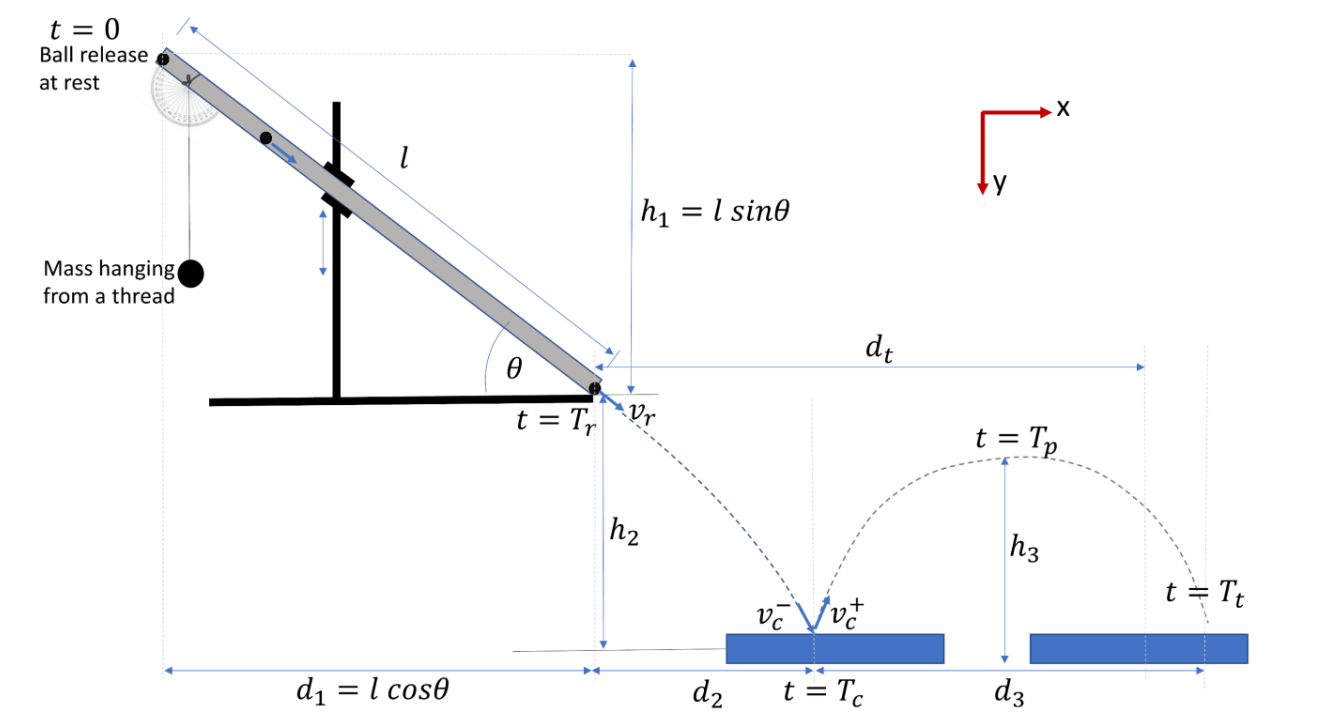
\includegraphics[width=1\linewidth]{Gamesetup.png}
    \caption{Game Setup}
    \label{fig:game_setup}
\end{figure}

\section{Methods}
    The total game setup can be separated into three sections:
    \begin{itemize}
        \item Sliding Down the Tube
        \item First Free Fall
        \item Bounce and Projectile motion
    \end{itemize}
    These sections use the method of conservation of energy, SUVAT equations, coefficient of restitution, and friction to compute the theoretical value of the horizontal distance to the location of the second bounce $d_t$ from the lower end of the tube.
    
    \subsection{Sliding Down the Tube}
        In the first section, the purpose is to determine the dropping velocity of the ball $v_r$, which is the velocity where the ball has just left the PVC tube. This could be computed by considering the following assumptions:
        \subsubsection{Assumptions}
            \begin{itemize}
                \item There is no friction acting between the sphere and the tube.
                \item The sphere will roll without slipping.
                \item The sphere's trajectory is a perfectly straight line down the tube.
                \item The sphere will not vibrate in the tube.
                \item The sphere is freely released, without any initial velocity.
                \item The sphere has no deformation during the motion.
                \item The air resistance is negligible in the tube.
                \item Energy is conserved.
                \item The gravitational acceleration constant is $9.81Nkg^{-1}$.
            \end{itemize}

    
        \subsubsection{Determination of the value of $v_r$}
            On this occasion, the conservation of energy can be determined as follows:
            \begin{equation}
                \Delta GPE = \Delta KE_t + \Delta KE_r \nonumber
            \end{equation}

        where $\Delta GPE$ is the change of gravitational energy, $\Delta KE_t$ is the change of kinetic energy, and $\Delta KE_r$ is the change of rolling kinetic energy. Due to the assumption above, the work done by the friction is negligible. Thus, the variables can be written as:
        \begin{itemize}
            \item $\Delta GPE = mgh$ 
            \item $\Delta KE_t = \frac{1}{2}mv^2$ 
            \item $\Delta KE_r = \frac{1}{2}I\omega^2 = \frac{1}{2}\cdot \frac{2}{5}mr^2\cdot\frac{v^2}{r^2} = \frac{1}{5}mv^2$ 
        \end{itemize}
        Thus 
        \begin{equation}
            \begin{aligned}
                mg\Delta h = \frac{1}{2}mv^2 + \frac{1}{5}mv^2 = \frac{7}{10}mv^2 \nonumber
            \end{aligned}
        \end{equation}
        In the first session of the experiment, the velocity is written as $v_r$ and the $\Delta h$ is written as $h_1$. Thus, the equation about $v_r$ and $h_1$ can be written as:
        \begin{equation}\label{vr}
            v_r = \sqrt{\frac{10gh_1}{7}}
        \end{equation}
        \subsubsection{Assumption effect}
            All the assumptions are based on the fact that there is no other energy lost. Thus the assumption will cause a higher predicted value of $v_r$ and larger than the actual value.
    \subsection{Free Fall}
    In the second section, the value of $d_2$ is determined by using the SUVAT equations and several assumptions.
        \subsubsection{Assumptions}
            \begin{itemize}
                \item The air resistance is negligible
                \item There is no additional rotational motion during the free fall.
                \item There is no external force acting on the system.
                \item The gravitational acceleration constant is $9.81 Nkg^{-1}$.
            \end{itemize}
        \subsubsection{Determine the horizontal and vertical component of the velocity}
            The horizontal and vertical force components of $v_r$ can be calculated as:
            \begin{equation}
                \begin{aligned}
                &v_{r_x} = v_rcos\theta  &v_{r_y} = v_rsin\theta
                \end{aligned}
            \end{equation}
        \subsubsection{Determination of the value of $t$ during free fall}
            According to the SUVAT equation $s = ut +\frac{1}{2}at^2$, The equation can be written as:
            \begin{equation}
                h_2 = v_{r_y}t + \frac{1}{2}gt^2 \nonumber
            \end{equation}
            This equation could be solved:
            \begin{equation}
                \begin{aligned}
                    t &= \frac{-v_{r_y}\pm\sqrt{{v_{r_y}}^2+2gh_2}}{g}\\
                      &= \frac{-v_{r}sin\theta\pm\sqrt{{v^2_{r}sin^2\theta}+2gh_2}}{g}\\
                \end{aligned}
            \end{equation}
        \subsubsection{Determination of the horizontal displacement $d_2$ during free fall }
            According to the SUVAT equation $s = vt$, the equation of $d_2$ can be written as:
                \begin{equation}
                    \begin{aligned}
                        d_2 &= vt
                        \\ &= \frac{v_rcos\theta \cdot (-v_{r}sin\theta\pm\sqrt{{v^2_{r}sin^2\theta}+2gh_2})}{g}
                    \end{aligned}
                \end{equation}
        \subsubsection{Assumption effect}
        The air resistance and rotational motion will cause external energy lost to the system. Thus the final $v_y$ and $v_x$ values will be smaller than the expected value.
    \subsection{First and Second Bounce}
        In the third section, the value of $d_3$ is determined using the SUVAT equations, Newton's law of restitution, and several assumptions.
        \subsubsection{Assumptions}
            \begin{itemize}
                \item There is no collision time.
                \item There is no air resistance.
                \item There is no friction between the ball and the ground.
                \item There is no rotational motion during the route.
                \item The coefficient of restitution is constant.
                \item The coefficient of restitution applies only to the vertical component of velocity
                \item Energy is conserved.
                \item The gravitational acceleration constant is $9.81Nkg^{-1}$.
            \end{itemize}
        \subsubsection{Determination of the vertical component of the velocity before collision}
            By using the SUVAT equation $v = u + at$, the equation about ${v^-_c}_y$ can be written as:
            \begin{equation}
                \begin{aligned}
                    {v^-_c}_y &= {v_r}_y + gt\\
                    &= v_rsin\theta + (-v_{r}sin\theta\pm\sqrt{{v^2_{r}sin^2\theta}+2gh_2}) \\
                    &= \pm\sqrt{{v^2_{r}sin^2\theta}+2gh_2}
                \end{aligned}
            \end{equation}
        \subsubsection{Determination of the vertical component of the velocity after collision}
            The coefficient of restitution $e$ is used for the inelastic collision, the formula given is:
            \begin{equation}
                v_2 - v_1 = -e(u_2-u_1) \nonumber
            \end{equation}
            On the occasion of the experiment, the formula can be simplified to:
            \begin{equation} 
                v_y = -e\cdot u_y \nonumber
            \end{equation}
            which is 
            \begin{equation}
                \begin{aligned}
                    {v^+_c}_y = -e\cdot {v^-_c}_y
                \end{aligned}  
            \end{equation}
        \subsubsection{During the projectile motion}
        According to the assumptions, there is no energy lost during the projectile motion between the first and the second bounces. It can therefore be assumed that the vertical component of the ball's velocity before the second bounce is the same size but opposite in direction as the vertical component of the velocity after the first bounce. Thus, by using the SUVAT equation $v = u + at$, the time $t_p = (T_p - T_c)\times2 $ during the bounces can be determined as:
        $$-{v^+_c}_y = {v^+_c}_y - gt_p$$
        so 
        \begin{equation}
            \begin{aligned}
                t_p &= \frac{2{v^+_c}_y}{g}\\
                    &= \frac{\pm2e\sqrt{{v^2_{r}sin^2\theta}+2gh_2}}{g}
            \end{aligned}
        \end{equation}
        \subsubsection{Determination of the horizontal displacement $d_3$ during projectile}
        According to the assumption, the horizontal speed of the sphere remains constant after sliding out of the tube. It is given by the SUVAT equation that $d = vt$, so $d_3$ can be determined as:
        \begin{equation}
            \begin{aligned}
                d_3 &= v_{r_x}t_p\\
                &=  \frac{\pm2ev_rcos\theta\sqrt{{v^2_{r}sin^2\theta}+2gh_2}}{g}
            \end{aligned}
        \end{equation}
        \subsubsection{Assumption effect}
            All the assumptions are based on there is no external energy lost. However, it is hard to determine if there is an energy transfer from rotational kinetic energy to horizontal linear kinetic energy during the collision. Thus, it is hard to determine if the actual value of $d_3$ is larger or smaller than the expected value.
    \section{Results}
        \subsection{Result Calculation}
            The purpose of this experiment is to compute the horizontal distance to the location of the second bounce $d_t$ from the lower end of the tube, where $d_t = d_2 + d_3$. Thus, the equation for $d_t$ is:
            \begin{equation}\label{d_t}
                \begin{aligned}
                    d_t &= \frac{v_rcos\theta \cdot (-v_{r}sin\theta\pm\sqrt{{v^2_{r}sin^2\theta}+2gh_2})}{g}\\&+\frac{\pm2ev_rcos\theta\sqrt{{v^2_{r}sin^2\theta}+2gh_2}}{g} \\
                    &= v_rcos\theta \Big(\frac{-v_rsin\theta\pm(1+2e)\sqrt{{v^2_{r}sin^2\theta}+2gh_2})}{g}\Big)
                \end{aligned}
            \end{equation}
            The parameters provided are shown in the table. With the given equation $h_1 = lsin\theta$, it can be determined that $h_1 = lsin40^\circ$.
            \begin{table}[H]
                \caption {Given Parameters} \label{parameters} 
                \begin{center}
                    \begin{tabular}{cc}
                        \hline
                        Parameter & Value \\
                        \hline
                        $\theta$     & $40^\circ$     \\
                        $l$         & $1.5m$     \\
                        $e$         & $0.4979 \pm 0.0142$     \\
                        $h_2$        & $0.7m$     \\
                        $m$         & $8\times10^{-3}kg$     \\
                        \hline
                    \end{tabular}
                \end{center}
            \end{table}
            After the substitution of  $v_r = \sqrt{\frac{10gh_1}{7}}$, $h_1 = lsin40^\circ$ and given parameters, the value of $d_t$ can be determined:
            $$d_t = 1.839649037156224m = 184cm$$  
            Considering there is a deviation of $\pm 0.0142$ for the value of the coefficient of restitution $e$, two more values of $d_t$ are considered:
            \begin{align}
                &d_{t_{upper}} = 1.8754782758273496m = 188cm \nonumber\\
                &d_{t_{lower}} = 1.8038197984850983m = 180cm \nonumber
            \end{align}
            Thus, the final predicted $d_t$ is:
            \begin{equation}
                d_t = 184 \pm 4cm \label{ans:1}
            \end{equation}
    \subsubsection{Assumption Effect}
    According to the previous discussion, the predicted value of $d_2$ will be larger than the calculated value, but the value of $d_3$ is difficult to judge. Therefore the overall predicted value of $d_t$ will be lower than the calculated value.
    \subsection{Errors and Sensitive analysis}
    In addition to the given deviation of the coefficient of restitution $e$, other errors in the data may also lead to deviations in the final result. The purpose of this section is to analyse the impact of different values on the final result. The following table shows the parameters in which deviation might occur. A predicted deviation will assume these values and the final result will be computed.
    \begin{table}[H]
                \caption {Perdicted Deviation} \label{tb:deviation} 
                \begin{center}
                    \begin{tabular}{cc}
                        \hline
                        Parameter & Value contains deviation \\
                        \hline
                        $\theta$     & $40\pm0.1^ \circ$     \\
                        $l$         & $1.500\pm 0.001m$     \\
                        $e$         & $0.4979 \pm 0.0142$     \\
                        $h_2$        & $0.70\pm0.01m$     \\
                        \hline
                    \end{tabular}
                \end{center}
            \end{table}
    To calculate more efficiently, a program is coded (see appendix \ref{ad:code}).
    The calculated difference between the maximum and the minimum value is $0.09974425189644576$. So the final range of the predicted value of $d_t$ is:
    $$d_t = 183.965\pm9.974cm$$
    This value is slightly larger than the predicted answer in equation \ref{ans:1}. For further analysis, a graph is plotted by the 81 results generated by the code. 
    \begin{figure}[H]
        \centering
        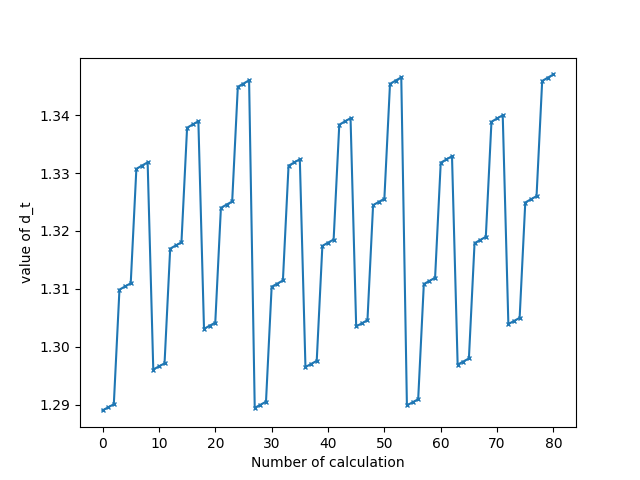
\includegraphics[width=0.75\linewidth]{code_output.png}
        \caption{the output of the code}
        \label{fig:code_output}
    \end{figure}
    In this plot, each of the three values ([0, 1, 2], [3, 4, 5]...) represents the impact of the error of $l$ on the data for the same $\theta$,$h_2$ and $e$. Every third number among each of the six values ([0, 3, 6], [1, 4, 7]...) represents the impact of the error of $e$ on the data for the same $\theta$,$h_2$ and $l$. Every third number among each of the nine values ([0, 9, 18], [1, 10, 19]...) represents the impact of the error of $h_2$ on the data for the same $\theta$,$l$ and $e$. Finally, every third number among each of the 27 values ([0, 27, 54], [1, 28, 55]...) represents the impact of the error of $\theta$ on the data for the same $e$,$h_2$ and $l$.The standard deviation of the whole data calculated is \textbf{0.03107009868988036}.\newline
    Thus, another code shown in Appendix \ref{code:p_error} is made for calculating the average percentage error. This can help determine which parameter affects the final value of $d_t$ most. With the output data, a table can be made:
    
    \begin{table}[H]
        \caption {Average Percentage Error} \label{tb:a_p_e} 
        \begin{center}
            \begin{tabular}{cc}
                \hline
                Parameter & Average uncertainty \\
                \hline
                $l$         & $0.855069\%$     \\
                $e$         & $1.950798\%$     \\
                $h_2$       & $0.707366\%$     \\
                $\theta$    & $0.000303\%$     \\
                \hline
            \end{tabular}
        \end{center}
    \end{table}
    It shows that the value of $e$ affects the $d_t$ most, where $\theta$'s percentage uncertainty is approximately zero. 
\section{Experiment Result}
    \begin{figure}[H]
        \centering
        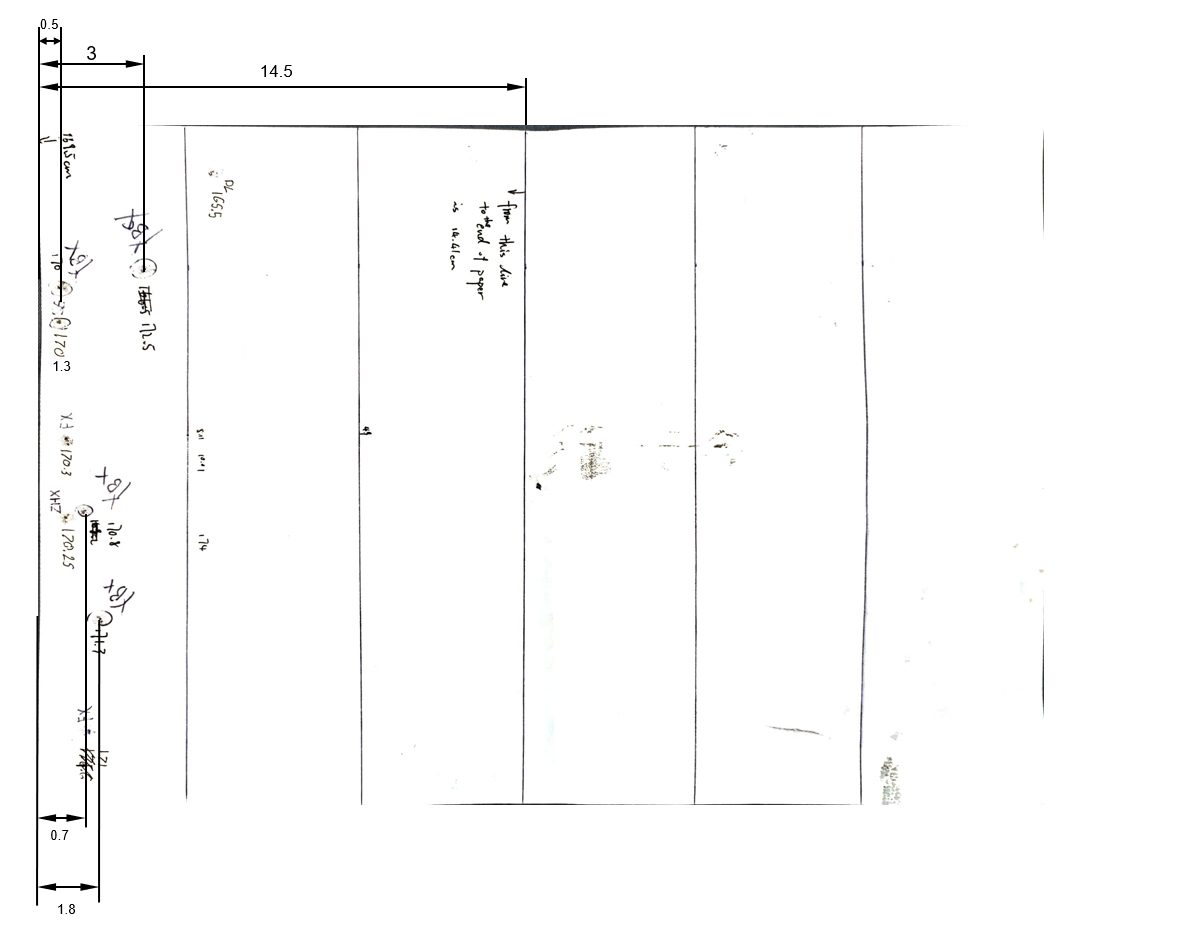
\includegraphics[width=1\linewidth]{experiment result.png}
        \caption{Experiment Result}
        \label{simplevr}
    \end{figure}
\section{Discussion}
    \subsection{Type of rotation of the metal ball}
        Three occasions might occur:
        \begin{itemize}
            \item Rolling without slipping
            \item Slipping
            \item Skidding
        \end{itemize}
        The first section of the ball can be seen as a ball on the slope, as shown below in Figure \ref{simplevr}, where $F_N$ is the normal force given by the slope, $f_s$ is the rolling friction force of the sphere, $F_G$ is the weight of the sphere, and $F_D$ is the component of gravity in the direction of the slope.
        \begin{figure}[H]
            \centering
            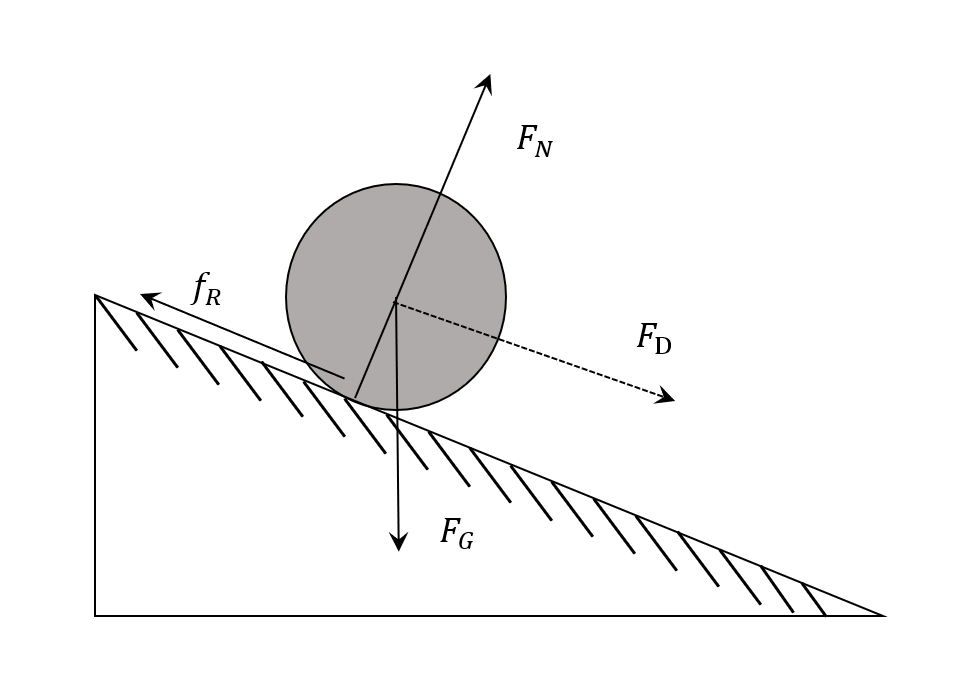
\includegraphics[width=0.5\linewidth]{simplized_rolling_resistance.png}
            \caption{Simplified force analysis of the sphere}
            \label{simplevr}
        \end{figure}
        Through this figure, we can derive the equation about the coefficient of static friction $\mu_{sphere}$ and the angle $\theta$ to satisfy rolling without slipping. It can be used to determine the maximum $\theta$ that can achieve rolling without slipping:
        \begin{equation}\label{Friction Required for Rolling Without Slipping}
        \begin{aligned}
            \theta = arctan(\frac{7}{2}\mu)
        \end{aligned}
        \end{equation}
        It is given that the maximum coefficient of static friction between the given material of stainless steel sphere and PVC tube $\mu$ is $0.53$ \cite{MechGuru}. By the equation \ref{Friction Required for Rolling Without Slipping}, the maximum angle $\theta$ can be computed:
        \begin{equation}
            \theta_{max} = arctan(\frac{7}{2}\times0.53) = 61.671^\circ
        \end{equation}
        It is given that $\theta$ for this experiment is $40\circ$, which is smaller than the calculated maximum value. Thus, the rotation status of the sphere could be determined as rolling without slipping, which means the assumption is \textbf{correct}.
    
    
    \subsection{Air Resistance during free fall}
During the free fall section, the sphere is at a relatively slow speed where there is turbulence, so the air resistance can be determined by the equation:
\begin{equation}
    F_d = -bv
\end{equation}
where:
\begin{itemize}
    \item $F_d$ is the air resistance
    \item $b$ is the constant that depends on both the material properties of the object and fluid, as well as the geometry of the object, and
    \item $v$ is the velocity
\end{itemize}
Due to Newton's Second law, a system of equations can be set:
\begin{equation*}
    \begin{cases}
    m\frac{dv_x}{dt} = -bv_x\\
    m\frac{dv_y}{dt} = mg-bv_y
    \end{cases}
\end{equation*}
After derivation (see equation \ref{y_air} and equation \ref{x_air} in appendix \ref{derviair} ), the equation set can be written as:
\begin{equation*}
    \begin{cases}
    v_x = v_0cos\theta\cdot e^{-\frac{bt}{m}}\\
    v_y = \frac{mg}{b} - e^{-\frac{tb}{m}}(\frac{mg}{b}-v_osin\theta)
    \end{cases}
\end{equation*}

Since the sphere is a relatively small object moving slowly through a viscous fluid, $b$ can be written as:
\begin{equation}
    b = 6\pi\eta r
\end{equation}
Thus these can be determined as
\begin{equation*}
   \begin{cases}
       v_x = v_0 cos\theta\cdot e^{-\frac{6\pi\eta tr}{m}}\\
       v_y = \frac{mg}{6\pi\eta r} - e^{-\frac{6t\pi\eta r}{m}}(\frac{mg}{6\pi\eta r}-v_osin\theta)
   \end{cases} 
\end{equation*}
In the air, the fluid viscosity is considered as $1.8\times10^{-5}kg/(ms^{-1})$.

\newpage
\appendix
\section{Appendices}
    \subsection{Proof of rolling without slipping occurs on a smooth slope} \label{proofofslide}
        The proof can be done by using the figure below:
        \begin{figure}[H]
            \centering
            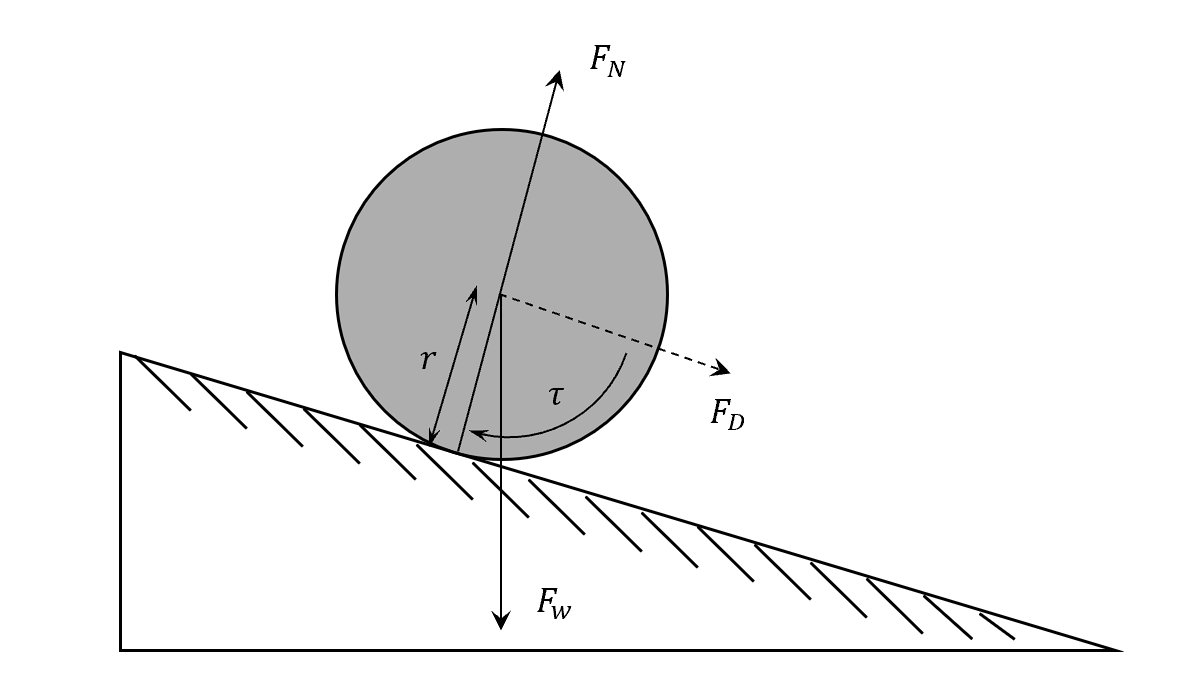
\includegraphics[width=0.5\linewidth]{no_friction.png}
            \caption{Simplified force analysis of the sphere on the smooth slope}
            \label{frictionless}
        \end{figure}
        In figure \ref{frictionless}, $F_N$ is the normal force acting on the slope, $F_W$ is the weight of the sphere, and $F_D$ is the component of gravity in the direction of the slope.
        By the formula of torque:
        \begin{equation}
            \tau = rFsin\theta
        \end{equation}
        There will be a torque $\tau$ equal to $F_dr$, which represents that the overall torque of the sphere is non-equilibrium. Thus, the sphere will \textbf{rotate}.
    \subsection{Derivation of Friction Required for Rolling Without Slipping} \label{deriviationofmu}
            This section shows how to derive the equation \ref{Friction Required for Rolling Without Slipping}.
            \begin{equation} 
            \begin{aligned} 
                \Sigma F = F_D - F_R = mgsin\theta - \mu\cdot mgcos\theta = ma\\
                \label{eq:user}
            \end{aligned}
        \end{equation}
        It is given that the acceleration of a sphere rolling down an incline is:
        \begin{equation}
            a_{sphere} = \frac{5}{7}gsin\theta
        \end{equation}
        Thus the minimum coefficient of static friction of the sphere to satisfy rolling without slipping could be determined as:
        \begin{equation}
            \begin{aligned}
                mgsin\theta - \mu \cdot mgcos\theta &= m\frac{5}{7}gsin\theta\\
                sin\theta - \mu\cdot cos\theta &= \frac{5}{7}sin\theta\\
                \mu &= \frac{2}{7}tan\theta\\
                \theta &= arctan(\frac{7}{2}\mu)\\
            \end{aligned}
        \end{equation}

    
    \subsection{Programme for computation of errors}\label{ad:code}
    \subsubsection{codes for $d_t$ values}
    \begin{python}
import numpy as np
"""
Declare all the variables
and consider some of their
deviation
"""
theta = [40-0.1,40,40+0.1] 
m = 0.008
h_2 = [0.7-0.01,0.7,0.7+0.01]
l = [1.500-0.001,1.500,1.500+0.001] 
g = 9.81
e = [0.4979-0.0142,
    0.4979,0.4979+0.0142] 
d = 0.0125
r = d/2
results = []

def get_vr(theta,l):
    """
    Calculate the value of vr and return
    its joining force and two components
    """
    h = l*np.sin(np.deg2rad(theta))
    vr = np.sqrt(10*g*h/7)
    vx = vr*np.cos(np.deg2rad(theta))
    vy = vr*np.sin(np.deg2rad(theta))
    return vr,vx,vy
    
def get_t(theta,h_2,l):
    """
    Calculate the value of t
    during the free fall.
    Ignore the non-possible values.
    """
    a = 0.5*g
    b = get_vr(theta,l)[2]
    c = -h_2
    t_1,t_2 = np.roots([a,b,c])
    if t_1 > 0 and t_2 > 0:
        return min(t_1,t_2)
    elif t_1 < 0 and t_2 < 0:
        raise ValueError
    else:
        return max(t_1,t_2)
        
def get_d2(theta,h_2,l):
    """
    Calculate the value of d2
    using the first two functions
    """
    t = get_t(theta,h_2,l)
    vr = get_vr(theta,l)[1]
    d2 = t*vr
    return d2
    
def get_dt(theta,h_2,e,l):
    """
    Calculate the value of d_3
    by the former functions and 
    return d_3 + d_2, which is 
    d_t
    """
    vry = get_vr(theta,l)[2]
    t = get_t(theta,h_2,l)
    vcy = vry + gt
    vcy_ = e * vcy
    Tp = vcy_ * 2 / g
    d_3 = get_vr(theta,l)[1] * Tp
    return d_3 + get_d2(theta,h_2,l)
    
def output(i,j,k,u):
    """
    Output all the values with
    appropriate description.
    """
    print("For theta = ",theta[i],
          "; h_2 = ",h_2[j],
          "; e = ",e[k],
          "; l = ",l[u],
          "; the value of d_t is"
          ,end=' ')
    result = get_dt(theta=theta[i],
                    h_2=h_2[j],
                    e=e[k],
                    l=l[u])
    results.append(result)

def print_graph():
    """
    plot a graph to determine which
    the parameter affects the most
    """
    import seaborn as sns
    import matplotlib.pyplot as plt
    import pandas as pd
    x = [x for x in range(len(results))]
    plt.plot(x, results)
    plt.show()

# main function for output     
for i in range(3):
    for j in range(3):
        for k in range(3):
            for u in range(3):
                output(i,j,k,u)
print_graph()
print(np.std(results)

    \end{python}
    \subsubsection{codes for percentage error}\label{code:p_error}
    \begin{python}
"""
Declaration of the list
of percentage errors
"""
p_error_e = []
p_error_theta = []
p_error_l = []
p_error_h_2 = []
def p_error(a,b,c):
"""
calculation of percentage error
"""
    return abs(100*(a+c-b-b)/(2*b))
for i in range(27):
    p_error_l.append(p_error
                    (results[i],
                    results[i+1],
                    results[i+2]))
    p_error_e.append(p_error
                    (results[i],
                    results[i+3],
                    results[i+6]))
    p_error_h_2.append(p_error
                       (results[i],
                        results[i+9],
                        results[i+18]))
    p_error_theta.append(p_error
                         (results[i],
                          results[i+27],
                          results[i+54]))
print(sum(p_error_l)/len(p_error_l))
print(sum(p_error_e)/len(p_error_e))   
print(sum(p_error_h_2)/len(p_error_h_2))  
print(sum(p_error_theta)/len(p_error_theta)) 
    \end{python}
    \subsection{Derivation of air resistance}\label{derviair}
        \subsubsection{Horizontal Component}
        For the horizontal component:
        \begin{equation}
            \begin{aligned}
                &m\frac{dv_x}{dt}= -bv_x\\
                &\int-\frac{b}{m}dt = \int\frac{1}{v_x}dv_x\\
                &-\frac{b}{m}t+c = ln |v_x|\\
                &v_x = e^{-\frac{b}{m}t}\cdot e^c = C_1e^{-\frac{bt}{m}}
            \end{aligned}
        \end{equation}
        It is given that when $t = 0$, $v_{0_x} = v_0cos\theta$, so:
        $$C_1 = V_0cos\theta$$
        Thus
        \begin{equation} \label{x_air}
            v_x = v_0cos\theta \cdot e^{-\frac{b}{m}t}
        \end{equation}
        \subsubsection{Vertical Component}
        For the vertical component:
        \begin{equation}
            \begin{aligned}
                m\frac{dv_y}{dt} &= mg-bv_y\\
                \int \frac{m}{mg-bv_y}dv_y &= \int dt\\
                -t + c &= \frac{m}{b}ln|mg-bv_y| \\
                e^{-\frac{tb}{m} + \frac{cb}{m}} &= mg-bv_y\\
                C_2\cdot e^{-\frac{tb}{m}} &= mg-bv_y\\
            \end{aligned}
        \end{equation}
        It is given that when $t = 0$, $v_{0_y} = v_0sin\theta$, so:
        $$C_2 = mg-bv_0sin\theta$$
        Thus
        $$(mg-bv_0sin\theta)\cdot e^{\frac{tb}{m}}(mg-bv_0sin\theta) = mg-bv_y$$
        so:
        \begin{equation} \label{y_air}
            v_y = \frac{mg}{b}-e^{-\frac{tb}{m}}(\frac{mg}{b}-v_0sin\theta)
        \end{equation}
        \subsubsection{Results}
        Thus, the horizontal component and the vertical component of the velocity can be written as:
        \begin{equation*}
            \begin{cases}
            v_x = v_0cos\theta\cdot e^{-\frac{bt}{m}}\\
            v_y = \frac{mg}{b} - e^{-\frac{tb}{m}}(\frac{mg}{b}-v_osin\theta)
            \end{cases}
        \end{equation*}
        
        
\section{Reference}
\printbibliography



\end{document}



